\section{简介}

\begin{figure}[H]
\centering

\includegraphics{img/logo.jpg}
\end{figure}
温故而知新。作业、考试、课外习题等不断产生错题,如何整理错题本?手抄,慢,花费时间长,很难坚持下去。剪贴,乱,可能需要额外复印空白题目。

你需要一个可以快速整理错题(拍照→剪切→涂改→保存),随时可以回顾复习的错题本app。\\

官网:\url{http://www.ycorb.com/}


\section{开始}
\subsection{打开}
\begin{figure}[H]
	\centering
	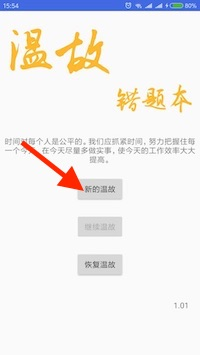
\includegraphics{img/1.jpg}
	\caption{首次打开}
	\label{img1}
\end{figure}
首次打开app,界面如图(\ref{img1})所示。点击“新的温故”进入数据初始化。

“恢复温故”使用请见后面\ref{restore}节。

数据初始化成功后,进入app初始默认页面,如图(\ref{img4})。
\begin{figure}[H]
	\centering
	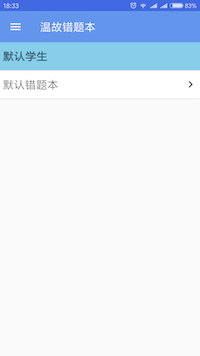
\includegraphics{img/4.png}
	\caption{默认页面}
	\label{img4}
\end{figure}

可以看到有一个默认学生,他有一本默认错题本。

\section{使用}
\subsection{学生管理}
支持多学生管理。低年级学生通常由家长帮助一起整理错题本,家里有多个孩子时适用。

点击左上角菜单,如图(\ref{img5}),打开侧边菜单,如图(\ref{img6})。
\begin{figure}[H]
	\centering
	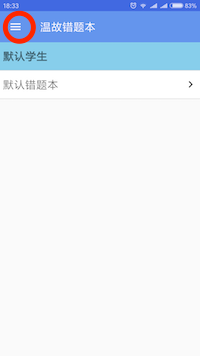
\includegraphics{img/5.png}
	\caption{侧拉菜单}
	\label{img5}
\end{figure}

\begin{figure}[H]
	\centering
	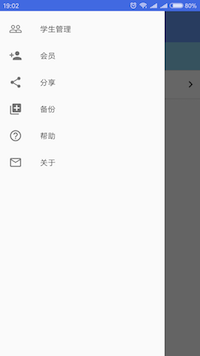
\includegraphics{img/6.png}
	\caption{菜单}
	\label{img6}
\end{figure}

点击“学生管理”,进入学生列表,如图(\ref{img7})。

\begin{figure}[H]
	\centering
	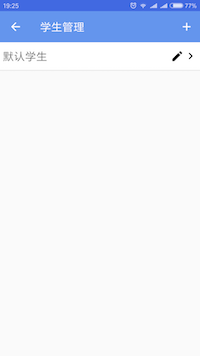
\includegraphics{img/7.png}
	\caption{学生列表}
	\label{img7}
\end{figure}

\subsubsection{增加学生}
我们这里新增加一个学生叫“小明”,点击右上角加号图标,如图(\ref{img8})。
\begin{figure}[H]
	\centering
	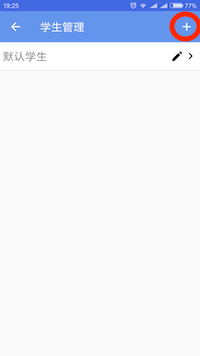
\includegraphics{img/8.png}
	\caption{+号图标}
	\label{img8}
\end{figure}

在文本框中输入“小明”,点击“增加”,如图(\ref{img9})
\begin{figure}[H]
	\centering
	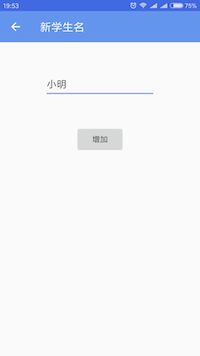
\includegraphics{img/9.png}
	\caption{增加学生}
	\label{img9}
\end{figure}

增加成功后,页面再次跳转到学生列表,如图(\ref{img10}),我们可以看到“小明”

\begin{figure}[H]
	\centering
	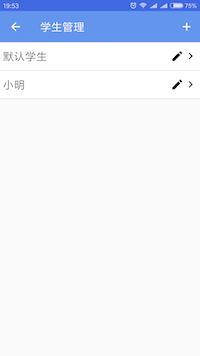
\includegraphics{img/10.png}
	\caption{学生列表}
	\label{img10}
\end{figure}

\subsubsection{修改学生名}
修改“默认学生”到“小红”,点击“默认学生”右侧的笔形图标,如图(\ref{img11})。
\begin{figure}[H]
	\centering
	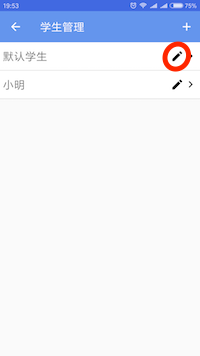
\includegraphics{img/11.png}
	\caption{笔形图标}
	\label{img11}
\end{figure}

进入修改页面,修改文本框中的“默认学生”到“小红”,点击修改按钮,如图(\ref{img12})。
\begin{figure}[H]
	\centering
	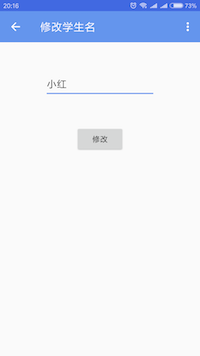
\includegraphics{img/12.png}
	\caption{修改到小红}
	\label{img12}
\end{figure}

修改成功后,页面跳转到学生列表,可以看到“默认学生”变成了“小红”,如图(\ref{img13})。
\begin{figure}[H]
	\centering
	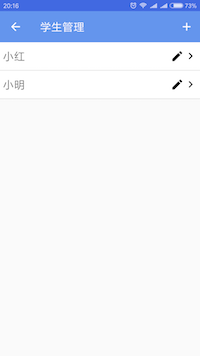
\includegraphics{img/13.png}
	\caption{学生列表}
	\label{img13}
\end{figure}

\subsubsection{删除学生}
\label{delete_student}
在修改学生名字页面,点击右上角菜单,如图(\ref{img14})。
\begin{figure}[H]
	\centering
	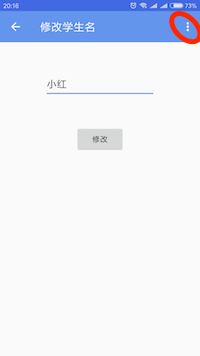
\includegraphics{img/14.png}
	\caption{删除学生}
	\label{img14}
\end{figure}

在菜单中,选择“删除”。注意:当此学生下面没有错题本时,才可删除。

\subsection{错题本管理}
\subsubsection{增加错题本}
我们现在给小红增加一个错题本“一年级数学(下)”。在学生管理--学生列表中找到小红,点击进入错题本管理,如图(\ref{img15}),可以看到,小红已经有一个“默认错题本”。
\begin{figure}[H]
	\centering
	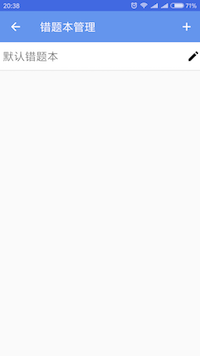
\includegraphics{img/15.png}
	\caption{错题本列表1}
	\label{img15}
\end{figure}

点击右上角加号图标,进入新错题本增加页面,完成增加后如图(\ref{img16})。
\begin{figure}[H]
	\centering
	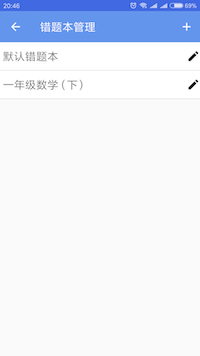
\includegraphics{img/16.png}
	\caption{错题本列表2}
	\label{img16}
\end{figure}

\subsubsection{修改错题本名}
修改小红的“默认错题本”到“一年级语文(下)”,在图(\ref{img16})中,点击“默认错题本”右侧的笔形图标,进入修改错题本名页面。修改完成后如图(\ref{img17})。
\begin{figure}[H]
	\centering
	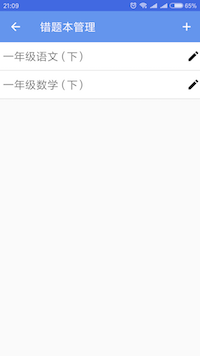
\includegraphics{img/17.png}
	\caption{错题本列表3}
	\label{img17}
\end{figure}

\subsubsection{删除错题本}
类似删除学生(\ref{delete_student}),也是在修改错题本名页面,点击右上角菜单。注意:当此错题本下所有错题全部复习完成,才可删除。